\section{What limits the advantage operationally}
\label{sec:limits}

DG's serial advantage is large, but five deployment
factors constrain it operationally.

\paragraph{1. Footprint.}

Both models are MoE with comparable footprints. Neither can share a GPU
with another large model. The asymmetry that matters is against the
quality-similar dense AR-1.5B at 3\,GB: sixteen copies fit in the
space either MoE model occupies.

\paragraph{2. Batching.}

Continuous batching converts arrival concurrency into throughput at
$25\times$ for AR-30B against $\leq 1.7\times$ for DG. We measured
DG on vLLM and LLaDA-8B on dInfer --- both engine-bounded stacks ---
so the true ceiling is unknown but lies at or above $1.7\times$. Even so, the gap is more
than an order of magnitude (Figure~\ref{fig:batching}); see
Appendix~\ref{app:batching}.

\begin{figure}[ht!]
\centering
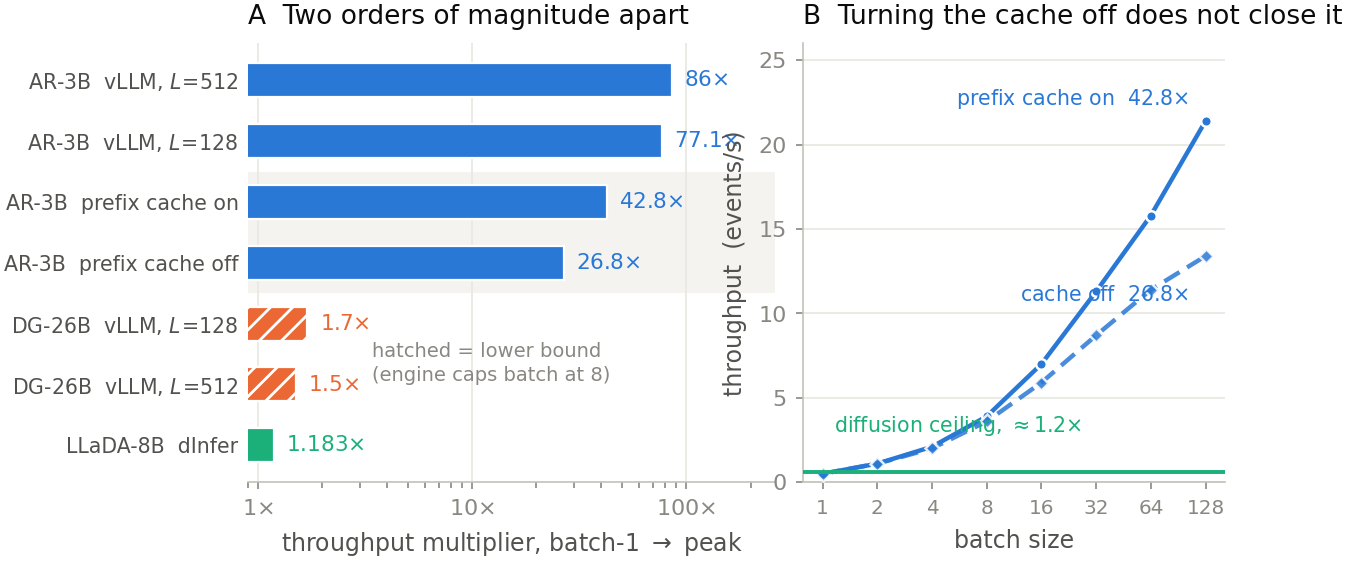
\includegraphics[width=\linewidth]{figures/fig6_batching.png}
\caption{Batch-1 to peak throughput multipliers. \textbf{A:} the AR-30B
MoE reaches $25\times$ via KV-cache reuse, while DG caps at
$\leq 1.7\times$ and LLaDA-8B on dInfer at $1.2\times$, two
diffusion families, two runtimes, the same ceiling, because
changing attention masks invalidate KV persistence across denoising
steps. \textbf{B:} turning the prefix cache off drops the dense AR-3B
only from \cacheOnMult$\times$ to \cacheOffMult$\times$, so prefix
sharing is not what creates the gap; KV persistence is. The cache
on/off and $L$-swept AR bars are the dense AR-3B, not the AR-30B MoE
(BGL, $n{=}300$).}
\label{fig:batching}
\end{figure}

\paragraph{3. Tail latency.}

DG arm's per-event coefficient of variation is \dgEventCV\%
with a max/median ratio of \dgMaxMed$\times$, against
\arEventCV\% and \arMaxMed$\times$ for the dense AR-3B, the only arm
measured per-event, since the AR-30B MoE was not re-run at that
granularity; see Appendix~\ref{app:distributions}.
A $3.21\times$ tail is what breaks a batch-1 SLA, exactly the
regime where DG's per-event advantage applies.

\paragraph{4. Input length.}

DG prefill slope is \inputSlopeRatio$\times$ steeper than
the dense AR-3B's (0.123 against 0.047\,ms per prompt token), because
each denoising step re-attends the full prompt. At
longer inputs the base rises and $L^{*}$ moves further upward; see
Appendix~\ref{app:input_canvas}, which also reports a canvas setting
that improves latency and quality at once.

\paragraph{5. Co-residency.}

If batch-1 is imposed by tenant isolation, sixteen copies of the
dense AR-1.5B (3\,GB each) fit in the same 52\,GB, preserving
isolation with $16\times$ the throughput --- a capacity projection,
not a measurement (linear scaling, no contention assumed).

\paragraph{Cost per event.}

Table~\ref{tab:cost} prices the comparison at a published on-demand
rate. The headline: at full duty, DG processes events at less than a
twentieth of a cent each. AR-30B costs two and a half times more. For a
business-to-business (B2B) log-processing service handling ten
thousand events per day, that is five dollars a day on DG versus
twelve on AR-30B, a \$2{,}600 annual gap on a single GPU.

\begin{table}[h]
\centering
\caption{Cost per event for three deployment arms at two duty cycles
(duty = fraction of wall-clock time the GPU is busy processing events).
DG is two and a half times cheaper per event than the AR-30B, because it
finishes an event in 379\,ms against 945\,ms. Each row prices a
single instance holding the whole GPU; sixteen co-resident AR-1.5B
copies would divide that rent sixteen ways, which is the comparison
the text draws below. GPU: A100 80GB PCIe at \$4.62/hr (AWS
p4de.24xlarge, August 2026).}
\label{tab:cost}
\begin{tabular}{@{}lrrrr@{}}
\toprule
Arm & Weights & Duty & Events/hr & \$/event \\
\midrule
AR-30B MoE (serial) & 60\,GB & 100\% & 3{,}810 & \$0.0012 \\
AR-30B MoE           & 60\,GB & 25\%  & 952 & \$0.005 \\
\midrule
AR-1.5B dense (one copy)    & 3.0\,GB & 100\% & 5{,}408 & \$0.0009 \\
AR-1.5B dense (one copy)     & 3.0\,GB & 25\%  & 1{,}352 & \$0.003 \\
\midrule
DG-26B-A4B (serial)  & 52\,GB & 100\% & 9{,}504 & \$0.0005 \\
DG-26B-A4B            & 52\,GB & 25\%  & 2{,}376 & \$0.002 \\
\bottomrule
\end{tabular}
\end{table}

Against the small dense arm instead of the MoE, that two-and-a-half-fold
advantage nearly vanishes:
\begin{equation}
R_{\mathrm{cost}} = \frac{\$ / \mathrm{event}_{\text{AR-1.5B}}}
{\$ / \mathrm{event}_{\textsc{dg}}}
= \frac{0.0009}{0.0005} = 1.8
\end{equation}
where both terms are the 100\%-duty single-copy rows of
Table~\ref{tab:cost}; the same ratio against the AR-30B is
$2.5\times$. Why does the much slower AR-1.5B nearly match DG on
cost? Because at 3\,GB it fits sixteen copies in one GPU, and
co-residency is parallelism by another name. Sixteen AR-1.5B instances
would produce $16 \times 5{,}408 = 86{,}528$ events/hr against DG's
9{,}504, a projection from the single-copy rate, not a measurement
making the co-resident deployment $9\times$ cheaper per event while
preserving tenant isolation. The takeaway: if you can batch, AR
wins on economics; if you can't, DG wins on latency.

